\begin{figure}[ht!]
\centering
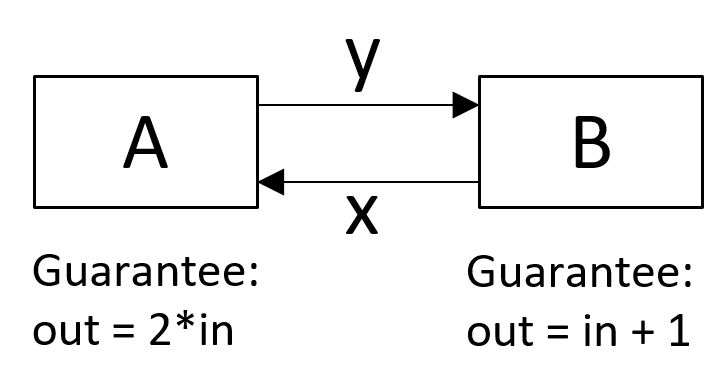
\includegraphics[width=40mm]{example1.jpg}
\caption{An AADL Model with AGREE Contracts\label{motivationFig1}}
\end{figure}

We use an example to explain the intuition and illustrate the key sematic difference between the synchronous MoC in original AGREE and the proposed scheduled dataflow MoC.
Consider an AADL model that consists of two threads $A$ and $B$, as shown in Figure \ref{motivationFig1}. Assume all ports are data ports. The behavior of each thread is indicated by its AGREE contract. Thread $A$ output doubles its input. Thread $B$ output increments its input by one. By the synchronous semantics, the value of signal $x = (x_1, x_2, ...)$ is defined by the solution to the fix-point equation $x = F(x)$, where $F(x) = 2x + 1$. That is, $x_1 = F(x_1), x_2 = F(x_2),...$. This results in $x = (-1, -1, -1,…)$. However, if the two threads execute in a sequential order $(A,B)^*$, given the initial value $x = 0$, an intuitive interpretation of the execution semanitcs is that $y_0 = 2x_0, x_1 = y_0+1, y_1 = 2x_1...$.That is, $x_1 = F(x_0), x_2 = F(x_1), x_3 = F(x_2),...$. This results in $x = (0, 1, 3, 5,…)$. The example shows the key difference between the two semantics in a model with cycles. In the synchronous model, the system behavior is defined by the solution(s) to a set of fix-point equations. While in the proposed MoC, the system behavior is defined through a sequence of executions.

\begin{figure}[ht!]
\centering
\includegraphics[width=80mm]{motivationalexample1.jpg}
\caption{An Example Model Illustrating Semantics\label{motivationFig2}}
\end{figure}

Now we use another example to illustrate the motivation of our work.
Consider an AADL model that consists of four threads $A, B, C, D$, as shown in Figure \ref{motivationFig2}. Assume all ports are data ports. Thread $A$ outputs the sequence of all natural numbers. Thread B and thread C simply copy its input to the output. Thread D is a subtractor, where the second (bottom) input value is substracted from the first (top) input value. Given a schedule $(ACABD)^*$, we want to prove that the primary output $x = (1,1,1,...)$. This can be achieved with the proposed modelling framework. However, it cannot be proved directly in the current AGREE framework, where the synchrnous semantics dictates $x= (0,0,0,...)$. A special construct \emph{delay} is often introduced to model execution order in a synchronous model. However, in the example, thread $B$ and $C$ essetially downsample the data stream from thread $A$. To model this kind of behavior, it requires much more complicated modelling mechanism than adding \emph{delays} in a synchornous model. 
Note that if the schedule is $(ABCD)^*$, then $x=(0,0,0,...)$. In fact, the whole system behavior is the same as that of the synchronous model. This also shows that the execution order could have an impact on the system behvavior. Therefore, a property proof has to be tied to a specific schedule.
Also note that we could add \emph{assumption: input is an even number} to thread $B$. The assumption has no impact on the system behavior under the proposed MoC. However, under the synchronous AGREE MoC the system has no valid behavior. This is because the assumption is violated under the synchronous semantics. This kind of assumptions are not uncommon. It creates a modelling challenge for using synchronous models. 

\begin{figure}[ht!]
\centering
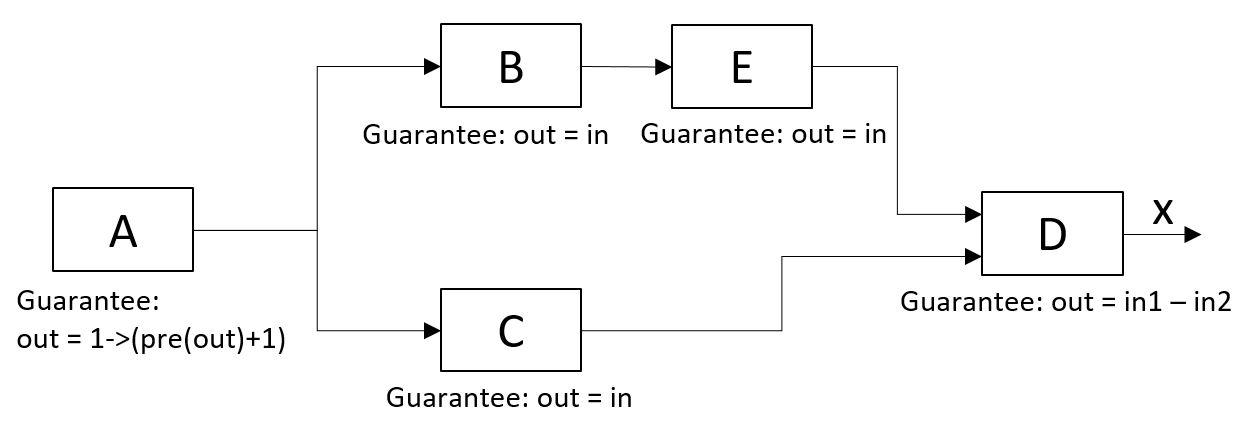
\includegraphics[width=100mm]{MotivationalExample2.jpg}
\caption{An AADL Model with AGREE Contracts\label{motivation1}}
\end{figure}
